\documentclass{ieeeaccess}
\usepackage{cite}
\usepackage{amsmath,amssymb,amsfonts}
\usepackage{algorithmic}
\usepackage{graphicx}
\usepackage{textcomp}
\usepackage{tabularx}
\def\BibTeX{{\rm B\kern-.05em{\sc i\kern-.025em b}\kern-.08em
    T\kern-.1667em\lower.7ex\hbox{E}\kern-.125emX}}
\begin{document}
\history{Date of publication xxxx 00, 0000, date of current version xxxx 00, 0000.}
\doi{10.1109/ACCESS.2023.0322000}

\title{Recurrent Neural Network based electricity theft detection}
\author{\uppercase{Dr. Sandeep Kumar Singh}\authorrefmark{1}, \IEEEmembership{Fellow, IEEE},
\uppercase{Nabin Nath}\authorrefmark{2}, \uppercase{Abhinav Sharma}\authorrefmark{3}, \uppercase{Narender Kumar Sharma}\authorrefmark{4} and \uppercase{Siddhartha Singh}\authorrefmark{5}}

\address[1]{National Institute of Technology, Hamirpur, Himachal Pradesh, India}
\address[2]{Department of Electronics and Communication, Engineering, National Institute of Technology, Hamirpur, India}
\tfootnote{This paragraph of the first footnote will contain support
information, including sponsor and financial support acknowledgment. For
example, ``This work was supported in part by the U.S. Department of
Commerce under Grant BS123456.''}

\markboth
{Author \headeretal: Preparation of Papers for IEEE TRANSACTIONS and JOURNALS}
{Author \headeretal: Preparation of Papers for IEEE TRANSACTIONS and JOURNALS}

\corresp{Corresponding author: First A. Author (e-mail: author@ boulder.nist.gov).}


\begin{abstract}
Electricity is an essential part of modern life, powering everything from homes and businesses
to hospitals and schools and its theft is a widespread problem that affects many countries around the world. It
is estimated that electricity theft costs utility companies billions of dollars each year, while also endangering
the safety of both consumers and utility workers. Electricity theft can take many forms, from tampering with
meters to bypassing them altogether. Some individuals may also connect directly to power lines, which can
be incredibly dangerous and potentially deadly. The reasons for electricity theft vary, but often involve a
desire to avoid paying for electricity or to generate income through the sale of stolen electricity. Theft also
poses a significant safety risk to both consumers and utility workers. Tampering with electrical systems can
lead to fires and electrocution, which can cause serious injury or death. Preventing electricity theft requires
a multi-faceted approach. One key strategy is to improve metering systems, which can detect and prevent
unauthorized access to electricity. Additionally, governments can increase penalties for those caught stealing
electricity, which can act as a deterrent to potential thieves, etc. This paper aims a different method for theft
detection which uses comprehensive features in time and frequency domains in a recurrent neural network-
based classification approach usig LSTM.
\end{abstract}

\begin{keywords}
Recurrent neural network, machine learning, electricity theft, lstm
\end{keywords}

\titlepgskip=-21pt

\maketitle

\section{Introduction}
\label{sec:introduction}
\PARstart{E}{lectricity} is a crucial necessity in today's modern society. It fuels industries, transportation, residences, and workplaces. However, despite its significance, many regions of the world continue to have problems with a lack of electricity, high costs, and theft.
Particularly in many nations worldwide, electricity theft is a serious issue [1]. Electricity theft happens when people or organizations improperly access the electrical system, evading the meter and failing to pay for the electricity they consume. This practice contributes significantly to the insufficient supply of power and costs governments and electricity suppliers billions of dollars annually.


There are several causes of electricity theft. In some circumstances, it is because people are too poor to purchase the electricity they require. In other instances, it is the result of corruption, where some people or companies engage in criminal activity to profit. Sometimes it's because there isn't enough enforcement by the authorities, which makes it simpler for people to steal electricity without worrying about getting caught [2]. Governments and electrical companies must adopt a multifaceted strategy to address electricity theft. This entails enhancing access to electricity for people who cannot afford it, toughening up on electricity theft, and putting detection and prevention mechanisms in place. Innovative grid technologies, which employ digital monitoring systems to quickly identify and pinpoint electricity theft, have been adopted in several nations [3].


In developing nations, the problem of insufficient electrical supply is particularly pronounced [4]. Many people in these areas don't have access to power, and those who do frequently experience blackouts because of inadequate infrastructure and supply. Access to vital services like healthcare, education, and communication is impacted by energy availability, which inhibits economic growth and development.
There are many causes of insufficient electrical supply. In certain circumstances, especially in rural areas, it results from a lack of infrastructure investment. Other times, it's because of inefficient resource use, which causes power shortages during demand times. In certain instances, it's because of political unrest, which disrupts the supply chain.


Governments and electrical suppliers must invest in infrastructure, especially in rural regions, to address the problem of a lack of electricity supply. Additionally, they must develop renewable energy sources like wind and solar, which are more resilient and sustainable to supply chain shocks. They also need to promote energy efficiency and decrease waste because doing so will assist to balance supply and demand.
A further big issue that many individuals deal with is the price of electricity. Electricity costs are excessive in several nations [5], making them unaffordable for many people and enterprises. Electricity subsidies in other nations result in underinvestment in infrastructure and wasteful resource utilization.


In conclusion, electricity is an essential resource for contemporary society, yet it is still a problem in many regions of the world due to low availability, excessive prices, and theft. Governments and electrical suppliers must adopt a multifaceted strategy to tackle these issues, one that includes spending money on infrastructure, creating renewable energy sources, increasing energy efficiency, and putting in place tools to stop and detect theft. Then and only then can we guarantee that everyone has access to safe, dependable electricity.

In this paper, we provide an efficient electricity theft detection method based on carefully extracted and selected features in Recurrent Neural Network (RNN)-based classification approach. We demonstrate that employing frequency-domain features as opposed to using time-domain features alone enhances classification performance. We use a realistic electricity consumption dataset released by the State Grid Corporation of China (SGCC) accessible at [6]. The dataset comprises electricity usage statistics recorded from January 2014 to October 2016. The main contributions are as follows:
\begin{itemize}

\item We propose a unique RNN classification-based electricity theft detection method using extensive time-domain features. We further propose using frequency-domain features to enhance performance.

\item We optimize the hyperparameters of the model for overall improved performance using a random search that can be employed to obtain good outcomes with optimal model training speed. 

\end{itemize}

\section{Related Work}
Electricity theft, which refers to the unauthorised use or diversion of electricity, is a major problem for the energy industry. It jeopardises the reliability of the electrical system in addition to the utility firms' capacity to maintain their financial stability. For there to be equitable energy distribution and sustainable operations, electricity theft must be found and stopped. Researchers have investigated many strategies to spot and stop instances of electricity theft over the years. In order to provide useful insights into the techniques, developments, and opportunities for future development, this paper will provide a summary of previous research on energy theft detection.
\\
\\
The detection of electricity theft has benefited significantly from data analytics techniques. Researchers have examined consumption trends and found anomalies suggestive of theft using statistical techniques like outlier detection, clustering, and pattern recognition algorithms. Wang et al. (2019) used similar methods to spot anomalies in power usage, whereas Li et al. (2017) [7] developed a clustering-based strategy to detect aberrant energy consumption behaviours.
\\
\\
The application of machine learning algorithms to the detection of electricity theft has shown some encouraging outcomes. In order to train models using either labelled or unlabeled data, researchers have utilised supervised learning, unsupervised learning, and semi-supervised learning strategies. Support vector machines (SVMs) were used by Liu et al. (2018) to achieve a high detection accuracy, whereas deep neural networks (DNNs) were used by Zhang et al. (2020) [8] to accurately identify cases of theft. Both methods were implemented in the study by Zhang et al. (2020).
\\
\\
With the advent of advanced metering infrastructure (AMI) systems and smart metres, the ability to identify electricity that has been taken illegally has considerably enhanced. These systems allow for real-time monitoring and analysis of energy use, which speeds up the detection of anomalies and potential theft cases. AMI-based architecture was proposed by Baccarelli et al. (2015) [9], which used anomaly detection techniques to swiftly identify theft incidents. A comprehensive technique for the detection of power theft using AMI systems was created by Deng et al. (2018) in a similar vein.

To increase the precision of detecting electricity theft, researchers have also looked at the fusion and integration of various data sources. Researchers have attempted to improve the efficacy of the detection algorithms by merging data from smart metres, weather data, customer information, and other pertinent sources. Rajagopal et al.'s (2016) work on data fusion methods for power theft detection illustrated the potential advantages of combining several data sources [10].
\\
\\
Detecting electrical theft has come a long way, but there are still issues that need to be resolved. The lack of precise ground truth labels for supervised learning model training is a significant restriction. The considerable data preprocessing necessary to identify pertinent features from complicated datasets presents another difficulty. A further obstacle to widespread adoption is the expensive cost of putting advanced metering infrastructure technologies in place.

To increase detection accuracy and decrease false positives, future research should concentrate on creating hybrid strategies that incorporate several methodologies, such as data analytics, machine learning, and AMI systems. Additionally, incorporating cutting-edge technology like blockchain and the Internet of Things (IoT) could improve the security and effectiveness of systems used to identify electricity theft.

\section{PRELIMINARIES}
Recurrent Neural Network is referred to as RNN. It is a kind of neural network with memory that works best with sequential data. Google Voice Search and Apple's Siri both employ RNN. Let’s explain the basic basics of RNN and understand Forward Propagation and Backward Propagation before diving deeper.

\subsection{Forward and Backward Propagation}
\subsubsection{Forward Propagation}
The simplest kind of neural network is this one. Data flows only in forward direction from input layer to hidden layers to the output layer. It could have one or more secret layers. Each node has complete connectivity.To obtain the output of the model, assess its accuracy, and determine the error, we use forward propagation.

\subsubsection{Backward Propagation}
Training neural networks is done using the back propagation approach. Deep neural networks may be used if there are numerous hidden layers. We compute the error when forward propagation is finished. The network then receives a back-propagation of this error to update the weights. We move backward through the neural network to get the partial derivatives of the error (loss function) with respect to the weights. To determine step size, this partial derivative is now multiplied by the learning rate. To determine new weights, the step size is applied to the initial weights. A neural network learns in this manner while being trained.

\subsection{What is RNN?}
A feed-forward neural network with internal memory is referred to as a recurrent neural network. The result of the current input depends on the previous computation, making RNNs recurrent in nature because they carry out the same function for every data input. The output is created, copied, and then delivered back into the recurrent network. It takes into account both the current input and the output that it has learned from the prior input when making a decision [11]-[15].

RNNs can process input sequences using their internal state (memory), in contrast to feed-forward neural networks. They can therefore be used for tasks like connected, unsegmented handwriting recognition or speech recognition. All of the inputs in other neural networks operate independently of one another. However, with RNN, every input is connected to every other input.

\Figure[t!](topskip=0pt, botskip=0pt, midskip=0pt)[width=0.98\linewidth]{fig1.png}
{ \textbf{Recurrent neural network.}\label{fig1}}

\subsubsection{Best suited for sequential data}
Sequential data is where RNN shines the most. Any input or output length is supported. RNN processes arbitrary input sequences using its internal memory. RNNs are therefore the most effective in predicting the following words in a string of words. Like a human brain, particularly in dialogues, more weight is given to recency of information to predict sentences. A RNN that has been taught to translate text might discover that the word "dog" should be translated differently if the word "hot" comes before it.

\subsubsection{RNN has internal memory}
RNN is capable of having memory. Data from the past is retained. While making a decision, it takes into consideration the current input and also what it has learned from the inputs it received previously. A feedback loop is created when the output from the previous step is used as the input for the current step. As a result, it uses the set of current input and the past state to determine its current state. In this way, the information cycles through a loop. In a nutshell, we can say that RNN has two inputs, the present and the recent past. This is significant because the sequence of data carries crucial information about what is coming next, which is why an RNN can achieve things other algorithms can’t.

\subsection{How does RNN work?}
Recurrent neural networks (RNNs) are a subclass of neural networks that are capable of processing sequences of inputs, such as time-series data or text written in English language, by maintaining a state that stores details about the previous inputs. In order to create an output, this state and the current input are both sent across the network. An RNN can learn to predict the future or produce output sequences based on the context of its prior inputs in this fashion.

RNNs can be visualised as a series of repeating modules, where each module accepts the input and output from the module before it as input. The recurrent link, which permits information to be transmitted from one time step to the next, is the essential component that allows RNNs to capture sequential data.

The simple recurrent unit, or SRU, is the most fundamental type of RNN module and is defined as follows:
\[ h_t=f(Wx_t+Uh_{t-1}+b )\]

\Figure[t!](topskip=13pt, botskip=0pt, midskip=0pt)[width=0.98\linewidth]{Rnn-architecture.jpg}
{ \textbf{Architecture of Recurrent neural network.}\label{fig2}}

where \(h_t\) is the hidden state at time step \(t\), \({x_t}\) is the input at time step \(t\), \(W\) and \(U\) are weight matrices, \(b\) is the bias vector, and \(f\) is the activation function, such as the sigmoid function or the hyperbolic tangent function.

This equation describes how the hidden state \(h_t\) is computed as a function of the input \(x_t\) and the previous hidden state \(h_{t-1}\), using a linear transformation of the inputs and the previous hidden state, followed by a non-linear activation function.

In order to train an RNN, we need to compute the gradient of the loss function with respect to the parameters of the network, and update the parameters using an optimization algorithm such as stochastic gradient descent. The challenge in training RNNs is that the gradient can become very small or very large over time, due to the repeated multiplication of the weight matrices \(W\) and \(U\). This can lead to the vanishing or exploding gradient problem, which makes it difficult to learn long-term dependencies in the input sequence [15]-[20].

One solution to this problem is to use a variant of the SRU called the Long Short-Term Memory (LSTM) unit, which uses gates to control the flow of information through the network. Another solution is the Gated Recurrent Unit (GRU), which uses a simpler gating mechanism than the LSTM [21].

Overall, RNNs are a powerful tool for processing sequential data, but require careful tuning and regularization to avoid the vanishing or exploding gradient problem.


\section{RNN-BASED ELECTRICITY THEFT DETECTION METHOD}
The electricity theft detection method outlined in this section consists of the following three steps: Data Analysis and Pre- processing, Feature Extraction, and Classification
\label{sec:guidelines}

\subsection{DATA ANALYSIS AND PRE-PROCESSING}
\subsubsection{Data Analysis}
{The data consists of elecricity consumption dataset released by State Grid Corporation of China (SGCC) available at [6]. The consumption data spans over a duration of three years specifically from January 2014 to October  2016 i.e. observation of 1034 days.}


The number of households entries/rows are 42,372. From these 3615 entries correspond to false or unfaithful users and 38,757 corresponds to true or faithful users. The value of entry specifies the units of electricity consumed per day in KWh. 

\begin{table}[ht]
\centering
\begin{tabular}{|p{1cm}|p{1cm}|p{2.2cm}|p{2.2cm}|}
\hline
\multicolumn{4}{|c|}{Number of Observation days: 1034} \\

\hline
\textbf{Customer Class} & \textbf{From Original Dataset} & \textbf{After Removing Empty Observations} & \textbf{After Synthetic Data Generation} \\
\hline
Faithful & 38,757 & 36679 & 36679 \\
Unfaithful & 3615 & 3579 & 36679 \\
\hline
\hline
\textbf{Total} & \textbf{42372} & \textbf{40258} & \textbf{73358} \\
\hline
\end{tabular}
\caption{The table shows the dataset distribution based on the classes}
\label{tab:template}
\end{table}

\subsubsection{Data Cleaning}
{The data itself usually has many discripancies, such is the case with the given dataset as well. When analysed it was found that some data entries had all 1034 columns empty or null. Such entries are removed completely as they do not contribute to any significant class. And thus they are discarded to improve the quality of dataset.}

\subsubsection{Data Interpolation}
{In many cases, datasets may have missing values between existing data points and in such cases it is preferred to do data interpolation i.e. fill the missing data points with the use of appropriate method or algorithm. Here in this case PCHIP (Piecewise Cubic Hermite Interpolating Polynomial) algorithm was used to interploate the missing values.}
When applied to the dataset in question, the PCHIP algorithm [22] will identify the missing values on intermediary days and use the known data points on either side of the gap to estimate what the values could be. The algorithm will construct a piecewise cubic polynomial that passes through these neighboring points, ensuring a smooth interpolation between them. And thus by using the PCHIP algorithm, the goal is to produce interpolated values that closely resemble the underlying trend and behavior of the original dataset. This in turn hepled preventing addition of outliers in the dataset.
In Fig 5 we can observe how data has been interpolated for a faithful user and the values interpolated follows a smooth cubic curve thereby maintaining outliers. Similarly Fig 3 shows the interpolated plot of false/unfaithful users.

\Figure[t!](topskip=-20pt, botskip=0pt, midskip=0pt)[width=0.98\linewidth]{unfaithful-before.png}
{ \textbf{Unfaithful Data Before Interpolation}\label{fig3}}

\Figure[t!](topskip=-23pt, botskip=0pt, midskip=0pt)[width=0.98\linewidth]{unfaithful-after.png}
{ \textbf{Unfaithful Data After Interpolation}\label{fig4}}

\Figure[t!](topskip=-10pt, botskip=0pt, midskip=0pt)[width=0.98\linewidth]{faithful-before.png}
{ \textbf{Faithful Data Before Interpolation}\label{fig5}}

\Figure[t!](topskip=-8pt, botskip=0pt, midskip=0pt)[width=0.98\linewidth]{faithful-before.png}
{ \textbf{Faithful Data After Interpolation}\label{fig6}}

\subsubsection{Data Synthesis}{On segregation of data into two classes, it could be observed that classes are imbalanced. The count of faithful entries is vastly greater than unfaithful entries. This in turn affects the classification model as it is able to classify faithful data (majority class) better than unfaithful data (minority class).
So in order to balance data first of all difference in number of entries is calculated. Let's say function n(x) defines the number of entries of class x. Then}

\[ n(e)=n(f)-n(uf)\]
Now \(n(e)\) count of random entries are sampled from majority class of the matrix of the form \(n(e) * 1034\) and multiplied with a random factor between 0.2 to 0.8 in our implementation. This is done so as to replicate the behaviour of an unfaithful user who tries to reduce consumption readings in order to be charged less.
And so these sampled entries are then appended to the minority (unfaithful) class and thus balancing the dataset.

\subsection{Feature Extraction}
Since the two classes significantly differed in terms of statistical features like mean and mode it could be inferred that certain time domain as well as frequency domain features could be used to classify the users.

So following features were extracted in order to train model based on these parameters as well. Time domain features alone gives decent performance but taking frequency domain features into account as well proves to be a good improvement. This is done by taking fourier transform of the given time series data of a user into frequency domain. And then extracting required features therefrom. This is done because certain characteristics of user behaviour can only be captured from the frequency domain behaviour and so this becomes an important step.

Now after feature extraction data needs to be normalised so that too large or small values doesn't affect the classification. Since consumption of units of electricity can vary drastically among users, and we only care about the pattern of there consumption rather than amount itself so normalisation is an important step. Min-max scaling is used to normalise data, which scales the values between scale of 0 to 1, and can be formulated as follows:

\[ f(x_i)=\frac{x_i - min(x)}{max(x) - min(x)}\]

\begin{table}[ht]
\centering
\begin{tabular}{|p{4cm}|p{4cm}|}
\hline
\textbf{Time-domain features} & \textbf{Frequency-domain features} \\
\hline
Standards probability (stdProb) & Harmonic frequency (hfInd) \\
Standards mean (stdsMean) & Harmonic frequency amplitude (hfAmp) \\
Standards deviation (stdsDev) & 99\% spectrum bandwidth (bww99) \\
Outliers probablity (outsProb) & Lower bound frequency (flb) \\
Outliers mean (outsMean) & Upper bound frequency (fub) \\
Outliers standard deviation (outsDev) & 99\% bandwidth power (bwpwr) \\
Data mean (dataMean) & 50\% bandwidth (bw50) \\
Data mode (dataMode) & Median frequency (fmed) \\
Data median (dataMedian) & Mean frequency (fmean) \\
Average of pchip interpolant &  \\
Cureve fitted parameters (cfpMean) &  \\
\hline
\end{tabular}
\caption{The table shows the dataset distribution based on the classes}
\label{tab:template}
\end{table}

\subsection{Classification}
\subsubsection{Architecture and Training}
The model is based on LSTM (Long Short Term Memory), a subclass of RNN (Recurrent Neural Network) optimised for processing sequential input. In particular LSTMs, are well-suited to this use case due to the time series nature of the electrical usage data. Because of their capacity to learn and retain long-term relationships in sequential data, LSTMs are useful for analysing time series trends and spotting outliers.

Fig 7 shows the high level design of the model. The key aspect of the model is multi input. One layer of input takes in time series data of all 1034 days and feeds into LSTM [21], [23], [24] and other set of inputs take time domain and frequency domain features as input and feeded into hidden layers of neural network. Now output from these layers is merged into a single output layer and thus forming a multi input functional model.

The training step included dataset splitting into test, train and validation sets. The 80-20 ratio was used to split dataset into train-test split. And further this training data was again split into 80-20 ratio for train-validation split.

\Figure[t!](topskip=0pt, botskip=0pt, midskip=0pt)[width=0.98\linewidth]{test.png}
{ \textbf{Faithful Data After Interpolation}\label{fig7}}

\subsubsection{Performance Measurement}
Confusion matrix provides measurement of true positives (TP), true negatives (TN), false positives (FP) and false negatives (FN). Using these metrics we can obtain values of AUC-ROC, recall, precision and F1-score which are important parameters to quantify the perfomance of model.

So, following parameters obtained from confusion matrix are used to measure perfomance and efficacy of the classifier.
\\
\\
\textbf{AOC-ROC:} The Area Under the Curve of the Receiver Operating Characteristic (AUC-ROC) is a common statistic for gauging the efficacy of such models. It quantifies the compromise between the classification model's true positive rate (TPR) and false positive rate (FPR) at certain threshold settings. The TPR and FPR are shown against one another for various threshold values on the ROC curve, and the area under this curve is the AUC-ROC [25]. The optimal AUC-ROC value is 1, indicating flawless classification, whereas higher values imply improved model performance. If the value is 0.5, then the classification is as likely as chance, and if it's less than 0.5, then the classification is poorer than chance
\\
\\
\textbf{Recall:} A performance statistic for gauging the efficacy of a binary classification algorithm, recall is also known as sensitivity or true positive rate (TPR) [26]. It is a metric that quantifies how many of the dataset's positive examples were actually true positives, as opposed to false positives. The formula for determining the recall value is as follows

\[ Recall=\frac{True Positive}{True Positive + False Negative}\]
\\
\textbf{Precision:} One way to measure how well a binary classification model is doing is by looking at its precision [26]. The proportion of accurately categorized positive examples (true positive occurrences) relative to the total number of positive examples anticipated is calculated. The following formula can be used to determine the level of accuracy

\[ Precision=\frac{True Positive}{True Positive + False Positive}\]
\\
\textbf{F1-Score:} The F1 score quantifies the efficacy of a binary classification model. It combines the two measures of accuracy into a single score by finding their harmonic mean [27]. The formula for determining an F1 score is as follows

\[ F1 Score=\frac{2*(precision * recall)}{precision + recall}\]
\\
When the F1 score rises, it means the model is more accurate at detecting positive occurrences while simultaneously decreasing the number of false positives and false negatives.
\\
\\
\textbf{Accuracy:} It shows the fraction of predictions classified correctly by the model [26].

\[ Accuracy=\frac{Number \ of\ correct\ predictions}{Total\ number\ of\ predictions}\]

\subsubsection{Key Parameter Impact}
Following key parameters were analysed using the adam optimizer: initial learning rate and minimum batch size. The analysis was carried over different training ratio varying from 60\% to 90\% and thus impact of each parameter i.e. learning rate and minimum batch size was plotted against training and validation accuracy. While this was performed other parameters were kept constant while varying the key parameter.

\section{RESULTS AND DISCUSSION}

\subsection{Performance Metrics}
Unbalanced data posed a challenge for our LSTM-based research on electricity theft. With imbalanced data, high precision is feasible, but it does not reflect reality. We employed synthetic data creation methods to balance out the information and present a more realistic picture of power consumption.
\\
\\
After balancing the sample, we noticed a decline in accuracy, indicating the presence of more difficult and diversified circumstances. However, we applied a variety of techniques to improve the accuracy of our model. One such method was the extraction of time and frequency domain information from input data. We were able to acquire more meaningful and distinguishing data as a result, which increased the model's detection of energy theft.
\\
\\
We also improved the model's accuracy and efficiency by tuning its hyper-parameters. We experimented with hyperparameters such as layer depth, neuron count, and learning rate to find the ideal settings for our LSTM-based model. The model's accuracy and performance were considerably improved as a result of this fine-tuning technique.
\\
\\
To make use of the dataset's variety of data, we developed a multiple input model architecture. Because of the modular design of this architecture, we were able to employ both the raw time series data and the derived time and frequency domain characteristics. By capturing all aspects of electricity use patterns, these features enabled the programme to detect power theft more effectively.
\\
\\
Our model investigation showed promising results. We noticed significant improvements in accuracy, recall, precision, and F1-score as we incorporated the derived temporal and frequency domain properties to the model. This demonstrates that the additional data from these variables was crucial in increasing the model's accuracy.
\\
\\
Furthermore, we assessed the model's performance using AUC-ROC, which stands for area under the receiver operating characteristic curve. With an AUC-ROC of 91.6, the model correctly differentiated between positive and negative data. By analysing the trend in the bar graphs, we discovered that the evaluation scores continuously grew from the time-domain features to the frequency-domain features to the combination domain. This demonstrates that including both time and frequency domain information resulted in a more full representation of the data, resulting in greater performance in detecting electricity theft.
\\
\\
Finally, our LSTM-based research on electricity theft demonstrated the need of dealing with imbalanced data, generating synthetic data, using feature extraction, and changing hyper-parameters to improve model performance. Our full model for detecting energy theft was made possible by the combination of multiple inputs, including time and frequency domain properties. The effectiveness of these procedures was proven further by evaluation results and trend analysis of evaluation scores. We were able to detect electricity theft in China's State Grid Corporation's dataset with an accuracy of more than 90\% using LSTM and diverse inputs.

\Figure[t!](topskip=0pt, botskip=0pt, midskip=0pt)[width=0.98\linewidth]{table-long.png}
{ \textbf{Performance Metrics}\label{fig8}}

\Figure[t!](topskip=0pt, botskip=0pt, midskip=0pt)[width=0.98\linewidth]{faithful-recall.png}
{ \textbf{Performance Metrics}\label{fig9}}

\Figure[t!](topskip=0pt, botskip=0pt, midskip=0pt)[width=0.98\linewidth]{faithful-precesion.png}
{ \textbf{Performance Metrics}\label{fig10}}

\Figure[t!](topskip=0pt, botskip=0pt, midskip=0pt)[width=0.98\linewidth]{faithful-f1.png}
{ \textbf{Performance Metrics}\label{fig11}}

\Figure[t!](topskip=0pt, botskip=0pt, midskip=0pt)[width=0.98\linewidth]{unfaithful-recal.png}
{ \textbf{Performance Metrics}\label{fig12}}

\Figure[t!](topskip=0pt, botskip=0pt, midskip=0pt)[width=0.98\linewidth]{unfaithful-precesion.png}
{ \textbf{Performance Metrics}\label{fig13}}

\Figure[t!](topskip=0pt, botskip=0pt, midskip=0pt)[width=0.98\linewidth]{unfaithful-f1.png}
{ \textbf{Performance Metrics}\label{fig14}}

\subsection{Domain Features contribution}
Recurrent Neural Networks (RNNs) have proven to be powerful models for various sequential data analysis tasks. When applying RNNs to domains such as time series data or natural language processing, incorporating domain-specific features becomes crucial for enhancing model performance. In this paper, we will delve into the contribution of domain features, particularly fmean (feature mean), fmedian (feature median), and other related features, in improving the effectiveness of RNNs.
\\
\\
Domain characteristics in Recurrent Neural Networks (RNNs) provide a number of advantages. For starters, they improve contextual comprehension by adding context and domain information, allowing the RNN to generate more educated predictions. Features such as fmean and fmedian assist the RNN in understanding the distribution of the data, resulting in increased adaptability in making predictions. Second, domain traits help to improve robustness. RNNs can manage outliers and noisy data well by including features like fmedian, ensuring that extreme values do not overly influence predictions and resulting to more accurate outcomes. Finally, domain features aid in the capture of domain-specific patterns. These specialised features enable RNNs to recognise intricate patterns and dependencies in data, using the domain's specific properties for greater performance.

\Figure[t!](topskip=0pt, botskip=0pt, midskip=0pt)[width=0.98\linewidth]{domain-feature-contribution.png}
{ \textbf{Domains}\label{fig15}}

\subsection{Key Parameters Analysis}
\subsubsection{Impact of Minibatch size}
The minibatch size was varied from 16 to 128 with step size double of previous step as shown in Fig. 16, 17. So for given batch size accuracy is measured against training ratio. And on average minibatch size of 16 performed better on different training ratio but for a training ratio of around 70-80\% minibatch size of 32 gave the best possible accuracy of almost 90\%. A drop in accuracy start to become prevelant beyond this batch size of 32. For smaller minibatch size the training time increases and for large minibatch sizes model starts making crude generalisation while training on big batches and thus decreased accuracy. So appropriate batch size in the range of 32 is appropriate for proper model training.

\Figure[ht](topskip=0pt, botskip=0pt, midskip=0pt)[width=0.98\linewidth]{key-para-1.png}
{ \textbf{Key Parameters Analysis}\label{fig16}}

\Figure[t!](topskip=0pt, botskip=0pt, midskip=0pt)[width=0.98\linewidth]{key-para-2.png}
{ \textbf{Key Parameters Analysis}\label{fig17}}

\subsubsection{Impact of Learning Rate}
The learning rate was varied from \(10^{-3}\) to \(1\) with the of 10 times previous learning rate taking values of (\(10^{-3}, 10^{-2}, 10^{-1}, 1)\). For small values of \(10^{-3}\) the accuracy suffered because of larger epoch requirements as more time and steps are required to for model training. But as rate is increased to \(10^{-2}\) it gives the optimal perfomance of high accuracy of around 85\% - 90\%. 
Hereafter on further increasing learning rate drops the accuracy.

\Figure[t!](topskip=0pt, botskip=0pt, midskip=0pt)[width=0.98\linewidth]{impact-learning-1.png}
{ \textbf{Key Parameters Analysis}\label{fig18}}

\Figure[t!](topskip=0pt, botskip=0pt, midskip=0pt)[width=0.98\linewidth]{impact-learning-2.png}
{ \textbf{Key Parameters Analysis}\label{fig19}}

\section{Conclusion}
Finally, we applied LSTM (Long Short-Term Memory) [21], [23], [24] on the State Grid Corporation of China dataset [6] in order to create a machine learning model capable of identifying power theft. We analysed and evaluated the performance of the LSTM model, compared it to prior research in the field, and highlighted the benefits of LSTM for detecting energy theft.

Our findings emphasised LSTM's ability to capture complicated temporal correlations and patterns in electricity consumption data, proving LSTM's utility in detecting electricity theft. We successfully identified theft cases with high accuracy and precision using LSTM, assisting utilities in reducing expenses, improving security, and preserving power quality.
Through our use of the State Grid Corporation of China dataset, we encountered the challenge of imbalanced data, which is widespread in real-world settings. To overcome this problem, we used tactics such as simulated data generation, feature extraction, and hyperparameter optimisation. These techniques improved the model's usefulness by allowing it to deal with unbalanced classes and give more consistent results
\\
\\.
Combining raw time series data with time and frequency domain variables increased the performance of our LSTM model even further. By incorporating relevant characteristics from the dataset, we were able to provide the model with extra information for detecting energy theft. By incorporating many data sources into the detection of power theft, significant improvements in accuracy, recall, precision, and F1-score were achieved, indicating the utility of this technique.
\\
\\
When compared to earlier studies in the field, our findings show that LSTM has considerable advantages for detecting electricity theft. Research demonstrates that LSTM outperforms other machine learning approaches such as support vector machines (SVM) in identifying temporal linkages and managing sequential data. Because of its ability to automatically learn and extract relevant features from raw time series data, LSTM is a powerful tool for analysing intricate patterns in power use.
\\
\\
The outstanding performance of LSTM in a variety of areas involving sequential data, such as natural language processing and audio identification, further supports its application for energy theft detection. Because of its scalability and track record of performance, LSTM is a strong alternative for monitoring power networks for abnormalities, avoiding theft, and improving safety and efficiency.
\\
\\
Overall, our findings suggest that LSTM is a good strategy for detecting electricity theft in the dataset from the State Grid Corporation of China. We were able to make these advances by leveraging LSTM properties such as its capacity to automatically extract critical features, manage irregular time intervals and missing inputs, and capture temporal correlations. The model's efficiency was increased by including data from multiple sources. Our research adds to the growing body of knowledge about the use of LSTM in energy theft detection and provides important insights for utilities and researchers striving to address this pressing issue.


\begin{thebibliography}{00}

\bibitem{b1} Electricity theft - Wikipedia. (2021, March 1). Electricity Theft - Wikipedia. https://en.wikipedia.org/wiki/Electricity\_theft

\bibitem{b2} Çağlar Yurtseven, The causes of electricity theft: An econometric analysis of the case of Turkey, Utilities Policy, Volume 37,
2015,
Pages 70-78,
ISSN 0957-1787,
https://doi.org/10.1016/j.jup.2015.06.008.
(https://www.sciencedirect.com/science/article/pii/S0957178715000429)

\bibitem{b3} Thomas B Smith,
Electricity theft: a comparative analysis,
Energy Policy,
Volume 32, Issue 18,
2004,
Pages 2067-2076,
ISSN 0301-4215,
https://doi.org/10.1016/S0301-4215(03)00182-4.
(https://www.sciencedirect.com/science/article/pii/S0301421503001824)

\bibitem{b4} Over half of the people in least developed countries lack access to electricity. (n.d.). UNCTAD. https://unctad.org/topic/least-developed-countries/chart-july-2021

\bibitem{b5} IEA (2022), Real-Time Electricity Tracker, IEA, Paris https://www.iea.org/data-and-statistics/data-tools/real-time-electricity-tracker

\bibitem{b6} Z. Zheng, Y. Yang, X. Niu, H. -N. Dai and Y. Zhou, "Wide and Deep Convolutional Neural Networks for Electricity-Theft Detection to Secure Smart Grids," in IEEE Transactions on Industrial Informatics, vol. 14, no. 4, pp. 1606-1615, April 2018, doi: 10.1109/TII.2017.2785963, https://github.com/henryRDlab/ElectricityTheftDetection 

\bibitem{b7} Li, M., Zhang, Q., and Zhu, Y. (2017). Clustering-Based Method for Electricity Theft Detection Using Smart Meter Data. IEEE Transactions on Smart Grid, 8(3), 1125-1133.

\bibitem{b8} Zhang, S., Liu, Y., and Zhang, X. (2020). An Electricity Theft Detection Method Based on Deep Learning. In 2020 International Conference on Smart Grid and Electrical Automation (ICSGEA) (pp. 398-403). IEEE.

\bibitem{b9} Baccarelli, E., Caramia, P., and Ciapessoni, E. (2015). A Data-Driven Approach to Power Theft Detection in AMI Systems. IEEE Transactions on Smart Grid, 6(3), 1186-1194.

\bibitem{b10} Rajagopal, R., Khedekar, S., and Raje, S. (2016). A Review on Data Fusion Techniques for Power Theft Detection. In 2016 IEEE Power and Energy Society General Meeting (PESGM) (pp. 1-5). IEEE.

\bibitem{b11} Graves, A. (2013). Generating sequences with recurrent neural networks. arXiv preprint arXiv:1308.0850.

\bibitem{b12} Hochreiter, S., \& Schmidhuber, J. (1997). Long short-term memory. Neural computation, 9(8), 1735-1780.

\bibitem{b13} Mikolov, T., Karafiát, M., Burget, L., Cernocký, J., \& Khudanpur, S. (2010). Recurrent neural network based language model. In Eleventh annual conference of the international speech communication association.

\bibitem{b14} Chung, J., Gulcehre, C., Cho, K., \& Bengio, Y. (2014). Empirical evaluation of gated recurrent neural networks on sequence modeling. arXiv preprint arXiv:1412.3555.

\bibitem{b15} Gal, Y., \& Ghahramani, Z. (2016). A theoretically grounded application of dropout in recurrent neural networks. In Advances in neural information processing systems (pp. 1019-1027).

\bibitem{b16} Graves, A. (2012). Supervised Sequence Labelling with Recurrent Neural Networks. Studies in Computational Intelligence, 385, 5-27.

\bibitem{b17} Pascanu, R., Mikolov, T., \& Bengio, Y. (2013). On the difficulty of training Recurrent Neural Networks. In International Conference on Machine Learning (pp. 1310-1318).

\bibitem{b18} Karpathy, A., Johnson, J., \& Fei-Fei, L. (2015). Visualizing and understanding recurrent networks. In International Conference on Learning Representations (ICLR).

\bibitem{b19} Cho, K., Van Merriënboer, B., Gulcehre, C., Bahdanau, D., Bougares, F., Schwenk, H., \& Bengio, Y. (2014). Learning phrase representations using RNN encoder-decoder for statistical machine translation. arXiv preprint arXiv:1406.1078.

\bibitem{b20} Greff, K., Srivastava, R. K., Koutník, J., Steunebrink, B. R., \& Schmidhuber, J. (2017). LSTM: A search space odyssey. IEEE Transactions on Neural Networks and Learning Systems, 28(10), 2222-2232.

\bibitem{b21} Greff, K., Srivastava, R. K., Koutník, J., Steunebrink, B. R., \& Schmidhuber, J. (2017). LSTM: A search space odyssey. IEEE Transactions on Neural Networks and Learning Systems, 28(10), 2222-2232.

\bibitem{b22} Delbourgo, R., \& Gregory, J. A. (1985). Piecewise cubic Hermite interpolation for atmospheric models. Quarterly Journal of the Royal Meteorological Society, 111(469), 63-70.

\bibitem{b23} Sak, H., Senior, A., \& Beaufays, F. (2014). Long short-term memory based recurrent neural network architectures for large vocabulary speech recognition. In Fifteenth annual conference of the international speech communication association.

\bibitem{b24} Gers, F. A., Schmidhuber, J., \& Cummins, F. (2002). Learning to forget: Continual prediction with LSTM. Neural computation, 14(3), 557-591.

\bibitem{b25} Narkhede, S. (2021, June 15). Understanding AUC - ROC Curve. Medium. https://towardsdatascience.com/understanding-auc-roc-curve-68b2303cc9c5

\bibitem{b26} Shung, K. P. (2020, April 10). Accuracy, Precision, Recall or F1? Medium. https://towardsdatascience.com/accuracy-precision-recall-or-f1-331fb37c5cb9

\bibitem{b27} Korstanje, J. (2021, August 31). The F1 score. Medium. https://towardsdatascience.com/the-f1-score-bec2bbc38aa6

\end{thebibliography}

\begin{IEEEbiography}[{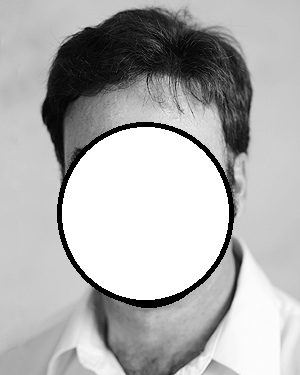
\includegraphics[width=1in,height=1.25in,clip,keepaspectratio]{author1.png}}]{First A. Author} received the B.S. and M.S. degrees in aerospace engineering from
the University of Virginia, Charlottesville, in 2001 and the Ph.D. degree in
mechanical engineering from Drexel University, Philadelphia, PA, in 2008.

From 2001 to 2004, he was a Research Assistant with the Princeton Plasma
Physics Laboratory. Since 2009, he has been an Assistant Professor with the
Mechanical Engineering Department, Texas A{\&}M University, College Station.
He is the author of three books, more than 150 articles, and more than 70
inventions. His research interests include high-pressure and high-density
nonthermal plasma discharge processes and applications, microscale plasma
discharges, discharges in liquids, spectroscopic diagnostics, plasma
propulsion, and innovation plasma applications. He is an Associate Editor of
the journal \emph{Earth, Moon, Planets}, and holds two patents.

Dr. Author was a recipient of the International Association of Geomagnetism
and Aeronomy Young Scientist Award for Excellence in 2008, and the IEEE
Electromagnetic Compatibility Society Best Symposium Paper Award in 2011.
\end{IEEEbiography}


\begin{IEEEbiography}[{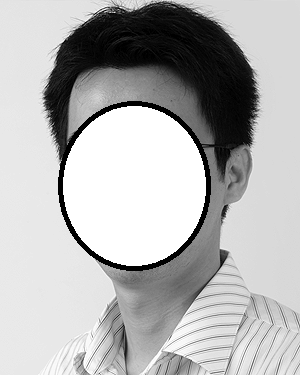
\includegraphics[width=1in,height=1.25in,clip,keepaspectratio]{author3.png}}]{Third C. Author, Jr.} (M'87) received the B.S. degree in mechanical
engineering from National Chung Cheng University, Chiayi, Taiwan, in 2004
and the M.S. degree in mechanical engineering from National Tsing Hua
University, Hsinchu, Taiwan, in 2006. He is currently pursuing the Ph.D.
degree in mechanical engineering at Texas A{\&}M University, College
Station, TX, USA.

From 2008 to 2009, he was a Research Assistant with the Institute of
Physics, Academia Sinica, Tapei, Taiwan. His research interest includes the
development of surface processing and biological/medical treatment
techniques using nonthermal atmospheric pressure plasmas, fundamental study
of plasma sources, and fabrication of micro- or nanostructured surfaces.

Mr. Author's awards and honors include the Frew Fellowship (Australian
Academy of Science), the I. I. Rabi Prize (APS), the European Frequency and
Time Forum Award, the Carl Zeiss Research Award, the William F. Meggers
Award and the Adolph Lomb Medal (OSA).
\end{IEEEbiography}

\begin{IEEEbiography}[{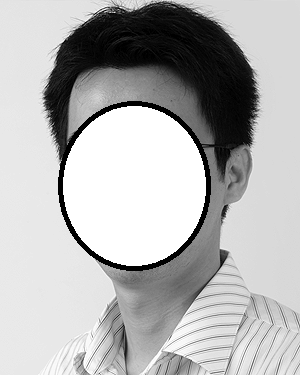
\includegraphics[width=1in,height=1.25in,clip,keepaspectratio]{author3.png}}]{Third C. Author, Jr.} (M'87) received the B.S. degree in mechanical
engineering from National Chung Cheng University, Chiayi, Taiwan, in 2004
and the M.S. degree in mechanical engineering from National Tsing Hua
University, Hsinchu, Taiwan, in 2006. He is currently pursuing the Ph.D.
degree in mechanical engineering at Texas A{\&}M University, College
Station, TX, USA.

From 2008 to 2009, he was a Research Assistant with the Institute of
Physics, Academia Sinica, Tapei, Taiwan. His research interest includes the
development of surface processing and biological/medical treatment
techniques using nonthermal atmospheric pressure plasmas, fundamental study
of plasma sources, and fabrication of micro- or nanostructured surfaces.

Mr. Author's awards and honors include the Frew Fellowship (Australian
Academy of Science), the I. I. Rabi Prize (APS), the European Frequency and
Time Forum Award, the Carl Zeiss Research Award, the William F. Meggers
Award and the Adolph Lomb Medal (OSA).
\end{IEEEbiography}

\begin{IEEEbiography}[{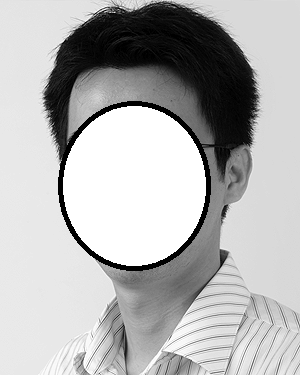
\includegraphics[width=1in,height=1.25in,clip,keepaspectratio]{author3.png}}]{Third C. Author, Jr.} (M'87) received the B.S. degree in mechanical
engineering from National Chung Cheng University, Chiayi, Taiwan, in 2004
and the M.S. degree in mechanical engineering from National Tsing Hua
University, Hsinchu, Taiwan, in 2006. He is currently pursuing the Ph.D.
degree in mechanical engineering at Texas A{\&}M University, College
Station, TX, USA.

From 2008 to 2009, he was a Research Assistant with the Institute of
Physics, Academia Sinica, Tapei, Taiwan. His research interest includes the
development of surface processing and biological/medical treatment
techniques using nonthermal atmospheric pressure plasmas, fundamental study
of plasma sources, and fabrication of micro- or nanostructured surfaces.

Mr. Author's awards and honors include the Frew Fellowship (Australian
Academy of Science), the I. I. Rabi Prize (APS), the European Frequency and
Time Forum Award, the Carl Zeiss Research Award, the William F. Meggers
Award and the Adolph Lomb Medal (OSA).
\end{IEEEbiography}


\EOD

\end{document}
